\documentclass[a4paper,parskip=half,ibliography=totocnumbered,titlepage]{scrartcl}

\usepackage[T1]{fontenc}  
\usepackage[utf8]{inputenc}
\usepackage[ngerman]{babel}
\renewcaptionname{ngerman}{\figurename}{Abb.}

\usepackage{multicol}         
\usepackage{mathtools}       
\usepackage{amssymb}
\usepackage{listings}      
\usepackage{csquotes}
\usepackage{pifont}

% Tabellen
\usepackage{booktabs}
\usepackage{multirow}
\usepackage{multicol}

\usepackage{tocloft}
\renewcommand{\cftfigpresnum}{Abb. }
\settowidth{\cftfignumwidth}{Abb. 10\quad}


\usepackage{ifthen}
\newcommand{\forloop}[5][1]{%
\setcounter{#2}{#3}%
\ifthenelse{#4}{#5\addtocounter{#2}{#1}%
\forloop[#1]{#2}{\value{#2}}{#4}{#5}}%
{}}

\newcounter{crcounter}

\newcommand{\compensaterule}[1]{%
\forloop{crcounter}{1}{\value{crcounter} < #1}%
{\vspace*{-\aboverulesep}\vspace*{-\belowrulesep}}}

\newcommand{\multirowbt}[3]{\multirow{#1}{#2}%
{\compensaterule{#1}#3}}


% bibtex
\usepackage[natbib,bibencoding=auto,style=authoryear,backend=biber]{biblatex}
\bibliography{references.bib}
\DeclareLanguageMapping{ngerman}{ngerman-apa}


%Schusterjungen und Hurenkinder
\clubpenalty = 10000
\widowpenalty = 10000

%Farbnamen benutzen
\usepackage[usenames,dvipsnames]{color}

\definecolor{black}{gray}{0} % Umdefinition der Farbe black, falls noetig (0=schwarz, 1=weiss)
\definecolor{dblue}{rgb}{0.1,0.2,0.6} % Dunkelblau, fuer Hyperlinks
\definecolor{lgray}{gray}{0.9} % Hellgrau, fuer Tabellen (0=schwarz, 1=weiss)
\usepackage[hyperfootnotes=false,colorlinks=true,linkcolor=black,citecolor=dblue,urlcolor=dblue]{hyperref} 

\usepackage{setspace}

\usepackage{enumitem}
\setlist{noitemsep} % or \setlist{noitemsep} to leave space around whole list

% \begin{enumerate}[label=(\roman{*})]

\newcommand{\HRule}[1]{\rule{\linewidth}{#1}} 	% Horizontal rule

\makeatletter							% Title
\def\printtitle{%						
    {\centering \@title\par}}
\makeatother									

\makeatletter							% Author
\def\printauthor{%					
    {\centering \large \@author}}				
\makeatother							

\usepackage{lastpage}
\usepackage{fancyhdr}
\pagestyle{fancy}
\fancyhf{}
\renewcommand{\footrulewidth}{0.5pt}
\renewcommand{\headrulewidth}{0.5pt}


% ------------------------------------------------------------------------------
% Metadata (Change this)
% ------------------------------------------------------------------------------

%Kopf- und Fußzeile, jeweils links und rechts
\fancyhead[L]{Dokumentation}
\fancyhead[R]{A.R.C.S.}
\fancyhead[L]{Projekt C}
\fancyfoot[R]{Seite \thepage\ von~\pageref{LastPage}}

%Titelblat
\title{\normalsize \textsc{Dokumentation Projekt C} 	% Subtitle of the document
		 	\\[2.0cm]													% 2cm spacing
            \HRule{0.5pt} \\ [0.5cm]										% Upper rule + 0.5cm spacing
			\LARGE \textbf{\uppercase{A.R.C.S - Android Rubik's Cube Solver}}	% Title
			\HRule{0.5pt} \\ [0.5cm]								% Lower rule + 0.5cm spacing
			\large Stephan Halbritter (Matr.-Nr.: 2093970)\\
      Colin Sames (Matr.-Nr.: 2093044)\\
		}

\author{Betreuer: Prof.~Dr.~Plaß\\
    Media Systems (B.Sc.)\\
    Hochschule für Angewandte Wissenschaften Hamburg\\
}


\begin{document}
% ------------------------------------------------------------------------------
% Maketitle
% ------------------------------------------------------------------------------
\thispagestyle{empty}				% Remove page numbering on this page

\printtitle									% Print the title data as defined above
  	\vfill
\printauthor								% Print the author data as defined above
\newpage

\tableofcontents
\newpage

\section{Idee}  % sgelb 100%
Die grundlegende Idee ist simpel und mit drei Schritten erklärt:

\begin{enumerate}

  \item Nehme einen ungelösten \emph{Rubik's Cube}

  \item Lese seine Seiten über die Kamera eines Smartphones ein

  \item Folge den Anweisungen und löse den Würfel

\end{enumerate}

Hauptaugenmerk lag hierbei auf dem möglichst einfachen Einlesen der sechs
Würfelseiten mit den insgesamt 54 Farbflächen.

\section{Der Würfel}  % 100% sgelb

\begin{figure}[ht!]
  \centering
  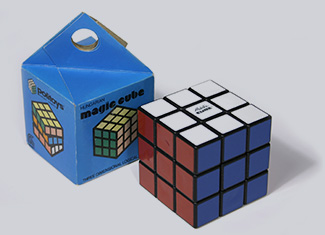
\includegraphics[width=\textwidth]{pics/rubikcube1977.jpg}
  \caption{Die ersten Exemplare wurden 1977 in Budapest verkauft
  (\cite{rubik:history})}
  \label{fig:rubik1977}
\end{figure}

Der \emph{Rubik's Cube} oder \emph{Zauberwürfel} wurde 1974 durch den
ungarischen Architekturprofessor Ernő Rubik erfunden, um seinen Studierenden
räumliche Verhältnisse anschaulicher präsentieren zu können. Seitdem beschäftigt
sich nicht nur die Mathematik immer wieder damit, der Würfel hat auch seinen
eigenen Sport, das \emph{Speedcubing} geschaffen.\footcite{rubik:history} 

\subsection{Aufbau}  % 100% sgelb

Der klassische sechsseitige Würfel aus Abbildung~\ref{fig:rubik1977} besteht aus
insgesamt 26 Teilen. Jede der sechs mittleren Flächen auf jeder Seite – die
\emph{Mittelteile} – hat eine eigene Farbe.\footnote{In der Regel sind dies
Orange, Blau, Rot, Grün, Weiß und Gelb} Sie lassen sich nicht rotieren, ihr
Position zueinander ist also festgelegt. Desweiteren gibt es zwölf
\emph{Kantensteine}, die zwei über eine Kante verbundene \emph{facelets}
verbinden und acht \emph{Ecksteine}, die drei \emph{facelets} über eine Ecke
verbinden.

\subsection{Lösungsalgorithmen}  % 100% sgelb

Insgesamt ergeben sich rund \( 4,3 \cdot {10}^{19} \) verschiedene
Kombinationen. Die maximale Anzahl von Zügen, um jeden beliebigen Würfel zu
lösen, wird \emph{God's number} genannt. Erst 2010 hat ein Team um Herbert
Kociemba durch ein Brute Force-Verfahren bewiesen, daß diese Nummer Gottes exakt
20 beträgt \citep{rubik:godsnumber}.

Zum Finden der optimalen Lösung kommt der \emph{Two-Phase}-Algorithmus zum
Einsatz. Dieser wurde erstmals von Herbert Kociemba vorgestellt
\citep{rubik:kociemba}. Wir nutzen Teile der optimierten Implementierung
von Shuang Chen, die er unter der GPLv3 auf github.com veröffentlicht
\citep{rubik:chen}.

\subsection{Notation}  % 100 % sgelb

Um die verschiedenen Züge, die es zur Lösung eines Würfels benötigt, zu
notieren, wird in der Regel auf folgendes Schema zurückgegriffen. Wenn nicht
anders angemerkt, wird sich auf eine Drehung um $90^\circ$ im Uhrzeigersinn
bezogen.

\begin{itemize}
  \item \textbf{F}ront bzw. Vorderseite
  \item \textbf{R}ight bzw. rechte Seite
  \item \textbf{B}ack bzw. Rückseite
  \item \textbf{L}eft bzw. linke Seite
  \item \textbf{D}own bzw. Unterseite
  \item \textbf{U}p bzw. Oberseite
  \item ein nachgestelltes Hochkomma \textbf{'} ändert die Rotationsrichtung gegen den
    Uhrzeigersinn
  \item eine nachgestellte \textbf{2} führt die Drehung zweimal, also um
    $180^\circ$ aus
\end{itemize}

Die Kombination \textbf{F2 B R' L} bedeutet also:
\begin{itemize}
  \item Drehe die Vorderseite um $180^\circ$
  \item Drehe die Rückseite um $90^\circ$ im Uhrzeigersinn
  \item Drehe die rechte Seite $90^\circ$ gegen den Uhrzeigersinn
  \item Drehe die linke Seite um $90^\circ$ im Uhrzeigersinn
\end{itemize}


\section{Umsetzung}  % sgelb 5/7%

\subsection{Bibliotheken und Tools}  % colin 0%
In diesem Kapitel werden die in diesem Projekt verwendeten Bibliotheken und
Hilfswerkzeuge vorgestellt.

\subsubsection{Java}  % 100%

Wenig überraschend wurde als Programmiersprache Java benutzt, das de facto den
Standard für die Androidprogrammierung darstellt.

\subsubsection{ADT/NDK}  % 100%

Ohne die \emph{Android Development Tools} und ihrer Vielzahl an in Eclipse
integrierten Tools wäre die Entwicklung nicht denkbar gewesen. Der Einsatz des
\emph{Native Development Kit} war notwendig, da das OpenCV SDK auf
C++-Bibliotheken aufbaut, über die so zugegriffen werden konnte.

\subsubsection{OpenCV}  % 100%

OpenCV ist eine in C und C++ geschriebene Bibliothek. Sie stellt eine große
Fülle an Funktionen zur Bildmanipulation und -erkennung zur Laufzeit zur
Verfügung. Mittels der \emph{OpenCV for Android
SDK}\footnote{\url{opencv.org/platforms/android.html}} wurden hiermit die Farben
der einzelnen Würfelflächen erkannt. Zum Einsatz kam OpenCV in der Version 2.4.9.

\subsubsection{Eclipse}  % 100%

Zur Programmierung haben wir auf Eclipse zurückgegriffen. Dafür sprachen mehrere
Gründe: zum damaligen Zeitpunkt war Eclipse die Standard-IDE zur
Androidentwicklung\footnote{Zumindestens nach Wünschen von Google soll diese
Rolle in Zukunft von \emph{Android Studio} eingenommen werden.}, das OpenCV SDK
war hierfür entwickelt worden und zu guter Letzt waren wir beide damit vertraut.

Eclipse bietet zudem die Möglichkeit, sehr einfach Tests mittels JUnit zu
schreiben. Tests sind sehr wichtig für dieses Projekt gewesen und haben mehrere
Male Fehler entdeckt, die leicht zu übersehen, auf längere Frist aber
schwerwiegend gewesen wären.

\subsubsection{Git}  % 100%

Als Versionsverwaltungssoftware haben wir Git gewählt, zur gemeinsamen
Codeverwaltung griffen wir auf GitHub zurück.

GitHub bietet zudem den Vorteil, dass es diverse Werkzeuge zur Projektplanung zur
Verfügung stellt. So ist es möglich, in einem Webinterface Milestones zu
definieren, Issues anzulegen und Aufgaben zuzuordnen. Das vereinfacht die
Planung ungemein.

Unsere Branching-Struktur folgt in einer vereinfachten Form dem Vorschlag von
Vincent Driessen \citep{git:driessen}: es gibt einen master-Branch, von dem aus
für vorher festgelegte Aufgaben (in Github \emph{Issues} genannt) ein Branch
erstellt wird. Ist die Aufgabe umgesetzt, wird der Branch wieder in den master
zurück gemergt. So bleiben die einzelnen Arbeiten voneinander getrennt, es gibt
mit master einen immer stabilen Zweig und das parallele Arbeiten gelingt zumeist
ohne Probleme.

Wir haben bewusst auf das EGit Plugin für Eclipse verzichtet. Stattdessen haben
wir auf das \emph{Ur-Git}, dem Kommandozeilenprogram, zurückgegriffen. Da beide
Projektmitglieder Linux zur Entwicklung nutzen, stellte das kein Problem dar.

\subsection{Gestaltung}  % sgelb 0%

Auch wenn die Gestaltung des Programmes nicht im Vordergrund stand, sollte die
Bedienung unkompliziert und nach Möglichkeit selbsterklärend sein. Es gibt zwei
Hauptansichten: eine für das Einlesen eines Würfels, eine für das Präsentieren
der Lösungsschritte (siehe Abbildung~\ref{fig:arcs_solving}). Der grundlegende
Aufbau der Oberfläche ist bei beiden der gleiche. Die Anzeige erfolgt im
Querformat. Auf der linken Seite wird eine Würfelseite angezeigt. Auf der
rechten Seite gibt konkrete Anweisungen für den User. Unter den Anweisungen
sind, leicht mit dem Daumen der rechten Hand zu bedienen, die notwendigen
Buttons angezeigt. Für die Darstellung wurde wenn möglich auf Standardelemente
der Android-API zurückgegriffen, das Einblenden der Kameransicht wurde über die
OpenCV-API realisiert.

\begin{figure}[ht!]
  \centering
  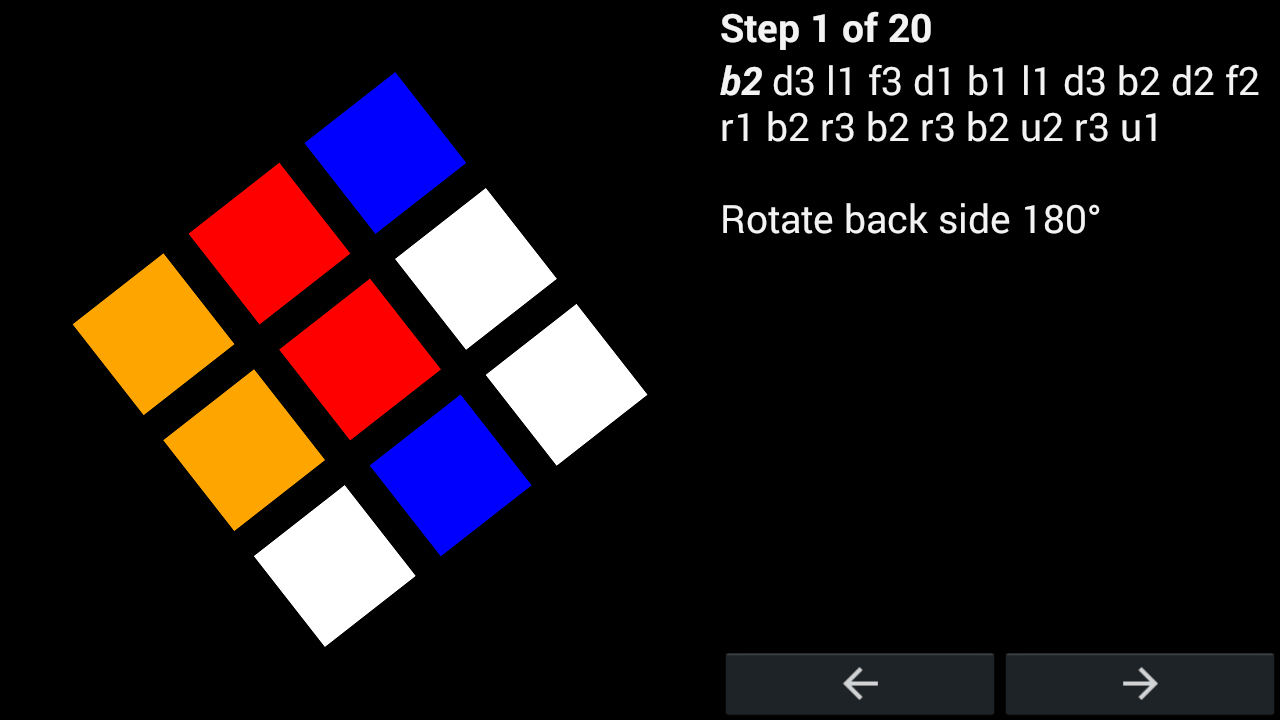
\includegraphics[width=\textwidth]{pics/arcs_solving.png}
  \caption{Ansicht des ersten Lösungsschrittes. Die Würfelansicht ist animiert.
  (Selbst erstellter Screenshot)}
  \label{fig:arcs_solving}
\end{figure}


\subsection{Arbeitsprozess}  % sgelb 0%

\section{Benutzerhandbuch}  % colin 0%

Die App A.R.C.S. ist eine App zur Lösung eines Rubiks Cube. Nach dem Starten der
App bekommt der User beim quer halten des Smartpones links das Kamerafeld und
rechts eine Beschreibung sowie einige Funktionen zu sehen. Auf dem Kamerafeld
links befinden sich 9 Quadrate. Der User hat die Wahl den Würfel mittels der
Kamera einzulesen, oder manuell. Möchte er dies automatisch tun, so hält er den
Würfel in die Kamera und achtet darauf, dass sich jedes Feld auf dem Würfel in
einem Quadrat auf dem Bildschirm befindet. Wie der User den Würfel halten muss,
wird mit einer Beschreibung rechts verdeutlicht. Zudem befindet sich über den 9
Quadraten ein Farblick makierter Strich, der zeigt, welche Farbe (mittleres Feld
des Würfels) oben liegen soll. Das Mittlere der 9 Quadrate ist auch Farblich
markiert. So kann eine eindeutige Position des Würfels ermittelt werden. Hat der
User den Würfel richtig positioniert, so kann er rechts auf einen Button
klicken, der die Farben des Würfels erkennt. Die Quadrate bekommen nun die
Farben der erkannten Felder. Sollte eine Farbe nicht richtig erkannt worden
sein, so kann er entweder erneut den Button betätigen oder manuell die Farbe
ändern indem er auf das Quadrat klickt. Der User bekommt nun eine Liste mit 9
Farben aus der er die gewünscht Farbe selektieren kann. Stimmen alle Farben, so
kann der User auf einen Butten mit einem "weiter" Pfeil drücken. Nun bekommt er
die nächste Seite des Würfels. Die Hinweise zur richtigen Ausrichtung des
Würfels sind für jede Seite angepasst. Möchte der User eine Seite zurück gehen,
so gibt es auch analog zum "weiter" Button auch einen "zurück" Button. Die
vorher eingelesenen Farben sind dort noch gespeichert und können editiert
werden. Nachdem der User alle Seiten eingelesen hat, kann er den Würfel mittels
eines Buttons auf der rechten Seite lösen lassen. Wurde der Würfel nicht rictig
eingelesen, so bekommt der User einen Hinweis das es z.B. nicht genau 9 Felder
von jeder Farbe gibt. Der User kann dann den Würfel nochmals überprüfen. Ist
alles richtig, so schaltet die App in den Lösungsmodus. Im Lösungsmodus hat der
User links die Felder wie sie nach einer Drehung aussehen sollten. Rechts hat er
eine Anleitung mit den Lösungsschritten. Jeder Schritt kann mit
Navigationsbuttons nacheinander aufgerufen werden. Nachdem der User alle
Schritte befolgt hat, sollte der Rubiks Cube gelöst sein.

\section{Architektur}  % colin 0%

\subsection{Hierarchie}  % 0%
Hier kommen die schicken UML-Diagramme unter.

\subsection{Prinzipien}  % 0%
das übliche OO-Blabla

\section{Auswertung und Fazit}  % sgelb 0%

Es ist uns gelungen, die gesetzten Ziele umzusetzen.




% Am Ende Bild- und Quellenverzeichnis
\appendix
\printbibliography[heading=bibintoc,title={Quellenverzeichnis}]
\listoffigures

\end{document}
